
% Preamble
\documentclass[11pt]{article}

% Packages
\usepackage{amsmath}
\usepackage{mathtools}
\usepackage{ragged2e}
\usepackage [utf8]{inputenc}
\usepackage{blindtext}
\usepackage{wrapfig}
\usepackage{xcolor}
\usepackage {polski}
\usepackage{multicol}
\usepackage[a4paper, total={5.7in, 8in}]{geometry}
\usepackage{graphicx}
\usepackage{amstex}
\usepackage{csvsimple}
\usepackage{changepage}
\usepackage{enumitem}
\usepackage[english]{babel}
\usepackage{biblatex}
\usepackage{caption}
\usepackage{indentfirst}

% Document
\begin{document}
%    Nagłówek
    \begin{flushleft}
        Filip Krauz-Damski 267 681 \hfill Data wykonania ćwiczenia:\\
        Filip Kubecki 272 655 \hfill 25 marca 2024r\\
        \hfill Data sporządzenia sprawozdania:\\
        Grupa: Pon 13:15 \hfill 7 kwietnia 2024r\\
    \end{flushleft}
    \begin{center}
        \Large\textbf{Ćwiczenie 3.}\\
        \textbf{Pomiary rezystancji i impedancji}
    \end{center}
    \vspace{1cm}

%    Treść
    \section{Spis przyrządów}
    \par{
        Do wykonania ćwiczenia wykorzystano:
        \begin{itemize}
            \setlength\itemsep{0em}
            \item[-] Przenośny multimetr analogowy AX-7003
            \item[-] Multimetr cyfrowy Agilent 34401A
            \item[-] Oscyloskop cyfrowy Agilent DSO3062A
            \item[-] Generator funkcji Agilent 33220A
            \item[-] Zasilacz laboratoryjny symetryczny NDN DF1730SL20A
        \end{itemize}
    }
    \section{Przebieg i cele doświadczeń}
    Doświadczenie polegało kolejno na:
    \begin{itemize}
        \setlength\itemsep{0em}
        \item Sprawdzeniu nominalnej rezystancji wszystkich oporników przydzielonych przez prowadzącego,
        \item Zmierzeniu omomierzem rezystancji przydzielonych oporników w układzie dwupunktowym,
        \item Zmierzeniu omomierzem trzech oporników wzorcowych oraz zapisaniu ich klasy dokładności nadanej przez producenta,
        \item Zmierzeniu rezystancji opornika z radiatorem, używając do tego różnych przewodów w celu zaobserwowania różnic we wskazaniach,
        \item Zmierzeniu rezystancji własnych przewodów długich o małym polu przekroju, dużym polu przekroju oraz krótkich o dużym polu przekroju,
        \item Zmierzeniu rezystancji opornika z radiatorem, używając metody czteropunktowej w celu pominięcia oporów przewodów pomiarowych,
        \item Oszacowaniu maksymalnego napięcia oraz natężenia dla opornika z radiatorem(tak aby moc wydzielona nie przekraczała 50[W]), a także pozostałych rezystorów(aby moc wydzielona nie przekraczała 2[W]),
        \item Zestawieniu układu poprawnego pomiaru natężenia oraz napięcia, zmierzeniu kolejno napięcia i natężenia dla
        każdego z oporników w obydwu układach, a następnie wyliczeniu rezystancji na podstawie tych pomiarów,
        \item Wyznaczeniu rezystancji granicznej multimetru, w celu sprawdzenia metody pomiaru,
        \item Wyznaczeniu częstotliwości granicznych oraz napięć wyjściowych, w celu wyliczenia wartości składowych R, L, C,
    \end{itemize}

    \section{Wyniki pomiarów}
    \subsection*{Część 1 - Odczytywanie wartości rezystorów na stanowisku}
    \begin{center}
        \small{\textbf{Tabela 1}}
    \end{center}
    \begin{center}
        \csvreader[tabular = |c|c|c|,
            table head = \hline  \textbf{Typ opornika} & \textbf{Rezystancja[\boldmath$\Omega$]} & \textbf{Tolerancja[\%]} \\\hline,
%            table foot = \hline,
            late after line = \\\hline
        ]{Dane/Czesc1.csv}{}{
            \csvcoli & \csvcolii & \csvcoliii
        }
    \end{center}
    \subsection*{Część 2 - Pomiary rezystancji w układzie dwupunktowym}
    \begin{center}
        \small{\textbf{Tabela 2}}
    \end{center}
    \begin{center}
        \csvreader[tabular = |c|c|c|c|,
            table head = \hline  \textbf{Typ opornika} & \textbf{Wartość[\boldmath$\Omega$]} & \textbf{Zakres[\boldmath$\Omega$]} & \textbf{Niepewność[\boldmath$\Omega$]} \\\hline,
%            table foot = \hline,
            late after line = \\\hline
        ]{Dane/Czesc2.csv}{}{
            \csvcoli & \csvcolii & \csvcoliii & \csvcoliv
        }
    \end{center}
    \subsection*{Część 3 - Pomiary rezystancji miernikiem analogowym}
    \begin{center}
        \small{\textbf{Tabela 3}}
    \end{center}
    \begin{center}
        \csvreader[tabular = |c|c|c|c|c|c|,
            table head = \hline  \textbf{Typ opornika} & \textbf{Rezystancja[\boldmath$\Omega$]} & \textbf{Wartość[\boldmath$\Omega$]} & \textbf{Zakres[\boldmath$\Omega$]} & \textbf{Niepewność[\boldmath$\Omega$]} \\\hline,
%            table foot = \hline,
            late after line = \\\hline
        ]{Dane/Czesc3.csv}{}{
            \csvcoli & \csvcolii & \csvcoliii & \csvcoliv & \csvcolv
        }
    \end{center}
    \subsection*{Część 4 - Pomiary oporników wzorcowych metodą czteropunktowych}
    \begin{center}
        \small{\textbf{Tabela 4}}
    \end{center}
    \begin{center}
        \csvreader[tabular = |c|c|c|c|,
            table head = \hline  \textbf{Typ opornika} & \textbf{Wartość[\boldmath$\Omega$]} & \textbf{Zakres[\boldmath$\Omega$]} & \textbf{Niepewność[\boldmath$\Omega$]} \\\hline,
%            table foot = \hline,
            late after line = \\\hline
        ]{Dane/Czesc4.csv}{}{
            \csvcoli & \csvcolii & \csvcoliii & \csvcoliv
        }
    \end{center}
    \subsection*{Część 5 - Pomiary rezystancji opornika z radiatorem przy pomocy różnych przewodów}
    \begin{center}
        \small{\textbf{Tabela 5}}
    \end{center}
    \begin{adjustwidth}{-25pt}{}
    \begin{center}
        \csvreader[tabular = |c|c|c|c|c|,
            table head = \hline  \textbf{Typ przewodów} & \textbf{Wartość[\boldmath$\Omega$]} & \textbf{Zakres[\boldmath$\Omega$]} & \textbf{Rezystancja przewodów[\boldmath$\Omega$]} & \textbf{Niepewność[\boldmath$\Omega$]}\\\hline,
%            table foot = \hline,
            late after line = \\\hline
        ]{Dane/Czesc5.csv}{}{
            \csvcoli & \csvcolii & \csvcoliii & \csvcoliv & \csvcolv
        }
    \end{center}
    \end{adjustwidth}
    \subsection*{Część 10 - Pomiary rezystancji przy wykorzystaniu metody poprawnego pomiaru napięcia}
    \begin{center}
        \small{\textbf{Tabela 6}}
    \end{center}
    \begin{adjustwidth}{-50pt}{}
    \begin{center}
        \csvreader[tabular = |c|c|c|c|c|c|c|c|c|,
            table head = \hline  \textbf{Opornik[$\Omega$]} & \textbf{U[V]} & \textbf{I[mA]}
            & \textbf{\boldmath$rn_U$[V]}  & \textbf{\boldmath$rn_I$[mA]} & \textbf{R[$\Omega$]}
            & \textbf{$\Delta_s$[$\Omega$]} & \textbf{$\delta_s$[\%]} & \textbf{$u_c(R)$[$\Omega$]}\\\hline,
%            table foot = \hline,
            late after line = \\\hline
        ]{Dane/Czesc10.csv}{}{
            \csvcoli & \csvcolii & \csvcoliii & \csvcoliv & \csvcolv & \csvcolvi & \csvcolvii & \csvcolviii & \csvcolix
        }
    \end{center}
    \end{adjustwidth}

    \subsection*{Część 11 - Pomiary rezystancji przy wykorzystaniu metody poprawnego pomiaru prądu}
    \begin{center}
        \small{\textbf{Tabela 7}}
    \end{center}
    \begin{adjustwidth}{-10pt}{}
        \begin{center}
            \csvreader[tabular = |c|c|c|c|c|c|c|c|c|,
                table head = \hline  \textbf{Opornik[$\Omega$]} & \textbf{U[V]} & \textbf{I[mA]}
                & \textbf{\boldmath$rn_U$[V]}  & \textbf{\boldmath$rn_I$[mA]} & \textbf{R[$\Omega$]}
                & \textbf{$\Delta_s$[$\Omega$]} & \textbf{$\delta_s$[\%]} & \textbf{$u_c(R)$[$\Omega$]}\\\hline,
%            table foot = \hline,
                late after line = \\\hline
            ]{Dane/Czesc11.csv}{}{
                \csvcoli & \csvcolii & \csvcoliii & \csvcoliv & \csvcolv & \csvcolvi & \csvcolvii & \csvcolviii & \csvcolix
            }
        \end{center}
    \end{adjustwidth}
    \newpage
    \subsection*{Część 16 - Pomiar imedancji przy pomocy oscyloskopu oraz generatora funkcji}
    \begin{center}
        \small{\textbf{Tabela 8}}
    \end{center}
    \begin{center}
        \csvreader[tabular = |c|c|,
            table head = \hline  \textbf{Częstotliwość[Hz]} & \textbf{Napięcie PeakToPeek[mV]} \\\hline,
%            table foot = \hline,
            late after line = \\\hline
        ]{Dane/Czesc16.csv}{}{
            \csvcoli & \csvcolii
        }
    \end{center}

    \section{Analiza wyników}
    \subsection*{Część 1-2}
    Na podstawie pomiarów z części 1 i 2 możemy przeprowadzić analizę
    poprawności pomiarów z wartością podaną przez producenta. W tabeli
    poniżej zebrano najważniejsze dane potrzebne do tej analizy:
    \begin{center}
        \csvreader[tabular = |c|c|c|c|c|c|,
            table head = \hline  \textbf{\boldmath$R_{p}$[\boldmath$\Omega$]} & \textbf{\boldmath$R_{zm}$[\boldmath$\Omega$]} & \textbf{\boldmath$T_{R_p}$[\boldmath$\Omega$]} & \textbf{\boldmath$\Delta$[\boldmath$\Omega$]} & \textbf{\boldmath$u_b(R_p-R_{zm})$[\boldmath$\Omega$]} & \textbf{\boldmath$R_p-R_{zm}$[\boldmath$\Omega$]} \\\hline,
%            table foot = \hline,
            late after line = \\\hline
        ]{Dane/Czesc12wyniki.csv}{}{
            \csvcoli & \csvcolii & \csvcoliii & \csvcoliv & \csvcolv & \csvcolvi
        }
    \end{center}
    {\footnotesize
        \begin{itemize}
            \setlength\itemsep{0em}
            \item[] \boldmath$R_p$ - rezystancja podana przez producenta,
            \item[] \boldmath$R_{zm}$ - rezystancja zmierzona miernikiem Agilent 34401A,
            \item[] \boldmath$T_{R_p}$ - tolerancja rezystora o rezystancji $R_p$ przeliczona na odpowiadając wartość w $\Omega$,
            \item[] \boldmath$\Delta$ - niepewność bezwzględna pomiaru rezystancji $R_{zm}$,
            \item[] \boldmath$u_b(R_p-R_{zm})$ - niepewność wynikająca z niepewności pomiarowej oraz tolerancji rezystora,
        \end{itemize}}
    Z tabeli można wywnioskować, że różnica między wartością podaną przez
    producenta a wartością zmierzoną miernikiem mieści się w zakresie
    niepewności szacowanej wynikającej z niepewności pomiaru oraz tolerancji rezystorów.\\
    Niepewność standardową typu B (niepewność szacowaną) obliczamy ze wzoru:
    \begin{gather*}
        u_b(x)=\sqrt{\sum_{i=1}^{n} \frac{\Delta_i^2}{3}}
    \end{gather*}
    {\footnotesize
        \begin{itemize}
            \setlength\itemsep{0em}
            \item[] \boldmath$\Delta_i$ - kolejne niepewności pomiarowe wynikające z urzadzeń pomiarowych, tolerancji elementów mierzonych, błędów eksperymentatora itp,
        \end{itemize}}
    Przykładowo dla rezystora 10[$\Omega$] na podstawie niepewności pomiarowej oraz tolerancji elementu:
    \begin{gather*}
        u_b(R_p-R_{zm})=\sqrt{\frac{\Delta^2}{3}+\frac{T_{R_p}^2}{3}}=\sqrt{\frac{(0.2033017[\Omega])^2}{3}+\frac{(0.001[\Omega])^2}{3}}=0.117377717[\Omega]\approx 0.12[\Omega]
    \end{gather*}

    Niepewność pomiaru rezystancji przy pomocy miernika Agilent 34401A przy pomocy metody dwupunktowej (2W) bez
    wykorzystywania funkcji \textbf{\textit{NULL}} obliczamy ze wzoru:
    \begin{gather*}
        \Delta=\pm(\alpha\%\cdot rdg + c\%\cdot rng + 0.2)
    \end{gather*}
    {\footnotesize
        \begin{itemize}
            \setlength\itemsep{0em}
            \item[] \boldmath$\alpha$ - współczynnik podany przez producenta który wymnażamy przez odczyt,
            \item[] \textbf{rdg} - wartość odczytana,
            \item[] \textbf{c} - współczynnik podany przez producenta który wymnażamy przez zakres,
            \item[] \textbf{rng} - zakres na którym zmierzono wartość/największa wartość jaką da się zmierzyć na zakresie,
        \end{itemize}}
    Przykładowo dla rezystora wzorcowego o wartości 10[$\Omega$]:
    \begin{gather*}
        \Delta=\pm(0.003\%\cdot 10.057 + 0.003\%\cdot 100 + 0.2)=0.2033017[\Omega]\approx 0.21[\Omega]
    \end{gather*}

    \subsection*{Część 3}
    Wyniki pomiarów pierwszych dwóch rezystorów (100[$\Omega$] i 6800[$\Omega$]) przy
    pomocy miernika analogowego wskazały poprawność pomiarów w granicy błędu pomiarowego miernika.
    W przypadku trzeciego rezystora o wartości 220 000[$\Omega$] wynik znacznie odbiegał od wartości
    podanej przez producenta i nie mieścił się w błędzie pomiarowym. \\
    \indent Wynika to z konstrukcji skali
    miernika (która wynika z zasady jego działania), która jest nieliniowa i pozwala na dokładny odczyt
    wartości z dolnego przedziału skali, lecz jej dokładność spada dla wartości najwyższych. W powyższym
    przypadku miernik nie pozwala na dokładne określenie wartości z zakresu od 100 000[$\Omega$] do 500 000[$\Omega$].
    Stąd niepoprawny wynik pomiaru.\\
    \newpage
    \noindent Niepewność pomiarową miernika analogowego AX-7003 obliczamy ze wzoru:
    \begin{gather*}
        \Delta=\frac{kl\cdot X_{max}}{100\%}
    \end{gather*}
    {\footnotesize
        \begin{itemize}
            \setlength\itemsep{0em}
            \item[] \boldmath$kl$ - klasa dokładności multimetra podawana w procentach,
            \item[] \boldmath$X_{max}$ - zakres pomiarowy/największa wartość możliwa do zmierzenia na zakresie,
        \end{itemize}}
   \noindent Przykładowo dla pomiaru rezystora o wartości 100[$\Omega$] przy pomocy miernika AX-7003:
    \begin{gather*}
        \Delta=\frac{5\%\cdot 10000}{100\%}=500[\Omega]
    \end{gather*}

    \subsection*{Część 4}
    Porównując wartości rezystancji z wartościami mierzonymi jesteśmy w stanie określić, że pomiary zostały przeprowadzone poprawnie.
    Metoda czteropunktowa pozwoliła na uzyskanie wyników o bardzo dużej dokładności jednak dla pewności porównamy różnicę między wartością
    podaną przez producenta a wartością zmierzoną a niepewnością typu b wynikającą z niepewności pomiarowej i tolerancji wykonania rezystorów:
    \begin{center}
        \csvreader[tabular = |c|c|c|c|,
            table head = \hline  \textbf{\boldmath$R_{p}$[\boldmath$\Omega$]} & \textbf{\boldmath$R_{zm}$[\boldmath$\Omega$]} & \textbf{\boldmath$R_{p}-R_{zm}$[\boldmath$\Omega$]} & \textbf{\boldmath$u_b(R_{p}-R_{zm})$[\boldmath$\Omega$]} \\\hline,
%            table foot = \hline,
            late after line = \\\hline
        ]{Dane/Czesc4wyniki.csv}{}{
            \csvcoli & \csvcolii & \csvcoliii & \csvcoliv
        }
    \end{center}
    {\footnotesize
        \begin{itemize}
            \setlength\itemsep{0em}
            \item[] \boldmath$R_p$ - rezystancja podana przez producenta,
            \item[] \boldmath$R_{zm}$ - rezystancja zmierzona miernikiem Agilent 34401A,
            \item[] \boldmath$u_b(R_p-R_{zm})$ - niepewność wynikająca z niepewności pomiarowej oraz tolerancji rezystora,
        \end{itemize}}
    Możemy zauważyć, że dla dwóch pierwszych pomiarów różnica wartości jest w granicy niepewności pomiarowej typu b.
    W przypadku trzeciego pomiaru różnica jest większa od niepewności typu b i wynosi ona jedynie
    0.0012[$\Omega$]. Wynika ona prawdopodobnie z błędnego przyjęcia
    że urządzenia były kalibrowane w przeciągu 24 h. Zmienia to współczynniki z który liczona jest
    Niepewność pomiaru miernikiem i może to zaniżać rzeczywistą niepewność z jaką miernik dokonuje pomiarów.\\
    W celu sprawdzenia tej tezy wyliczono niepewność typu b w przypadku niepewności
    liczonej ze współczynników dla multimetra kalibrowanego ponad 1 rok temu.
    Kalkulacja ta dla pomiaru rezystora 100[$\Omega$] dała nam niepewność typu b wynoszącą:
    \begin{gather*}
        u_b(R_p-R_{zm})=0.009932733773\dots[\Omega]\approx 0.010[\Omega]
    \end{gather*}
    \indent W tym przypadku więc różnica między wartościami rezystancji mieści się w zakresie niepewności typu b.
    Należałoby również zapytać opiekuna urządzeń w sali o okres, w jakim urządzenia są
    kalibrowane, aby wiedzieć jakie wartości przyjmować dla przyszłych obliczeń niepewności.\\\\
    \indent Niepewność pomiarową miernika Agilent 34401A przy
    metodzie czteropunktowej wyliczamy podobnie jak niepewność metody
    dwupunktowej wykorzystanej w części 2 jednak nie dodajemy do wyniku stałej 0.2[$\Omega$].
    Niepewność typu b również wyliczamy analogicznie jak w punkcie 2.

    \subsection*{Część 5-6}
    Wskazania omomierza dla różnych przewodów różnią się, ponieważ do pomiaru dodaje się rezystancja przewodów.
    Przewody mają różne rezystancje zależnie od ich długości i pola przekroju. Wynika to z zależności:
    \begin{gather*}
        R=\rho\cdot\frac{l}{S}
    \end{gather*}
    {\footnotesize
        \begin{itemize}
            \setlength\itemsep{0em}
            \item[] \boldmath$\rho$ - rezystywność materiału z jakiego zrobiony jest przewód,
            \item[] \boldmath$l$ - długość przewodu,
            \item[] \boldmath$S$ - pole przekroju poprzecznego przewodu,
        \end{itemize}}
    Dlatego przewody dłuższe i o małym polu przekroju będą zawyżały wynik bardziej niż przewody krótkie o dużym polu przekroju.
    Zauważamy to w pomiarach gdzie największą rezystancję zmierzono długimi przewodami o małym polu przekroju a najmniejszą
    rezystancję krótkimi przewodami o dużym polu przekroju.\\
    Aby zredukować wpływ rezystancji przewodów zmierzono rezystancję kolejnych przewodów zwierając je przy włączonym omomierzu
    i odczytując wyniki a następnie odejmując odczytaną wartość od wyniku pomiaru przy pomocy danych przewodów.
    Poniżej umieszczono tabelę podsumowującą te obliczenia:
    \begin{center}
        \csvreader[tabular = |c|c|c|c|,
            table head = \hline  \textbf{\boldmath$R_{p}$[\boldmath$\Omega$]} & \textbf{\boldmath$R_{zm}-R_k$[\boldmath$\Omega$]} & \textbf{\boldmath$R_{p}-(R_{zm}-R_k)$[\boldmath$\Omega$]} & \textbf{\boldmath$u_b(x)$[\boldmath$\Omega$]} \\\hline,
%            table foot = \hline,
            late after line = \\\hline
        ]{Dane/Czesc5wyniki.csv}{}{
            \csvcoli & \csvcolii & \csvcoliii & \csvcoliv
        }
    \end{center}
    {\footnotesize
        \begin{itemize}
            \setlength\itemsep{0em}
            \item[] \boldmath$R_p$ - rezystancja podana przez producenta,
            \item[] \boldmath$R_{zm}$ - rezystancja rezystora,
            \item[] \boldmath$R_k$ - rezystancja przewodów,
            \item[] \boldmath$u_b(x)$ - niepewność typu b wynikająca z niepewności pomiarowej rezystora, przewodów oraz tolerancji rezystora,
        \end{itemize}}
    \par Można zauważyć, że różnica między wartością oczekiwaną a wartością obliczoną jest mniejsza niż błąd pomiarowy z jakim
    została wyznaczona. Można więc uznać, że wartość wyznaczona jest w granicy błędu pomiarowego. W
    tabeli nr 5 można jednak zauważyć pewną nieścisłość z założeniami. Zgodnie ze wzorem na rezystancje przewodnika
    Krótkie przewody o dużym przekroju poprzecznym powinny posiadać najmniejszą rezystancję jednak w tym przypadku
    jest ona większa od rezystancji przewodów o długości 1 metr i dużym przekroju poprzecznym. Wynik przed odjęciem rezystancji
    przewodów jednak zachowują się zgodnie z przewidywaniami. \\
    \indent Powodem tej anomalii może być wymienianie się przewodami przez grupy
    eksperymentujące. Po wykonaniu pomiarów z części 5 przewody były pożyczane innym stanowiskom, gdyż sala nie posiadała wystarczającej ilości
    kompletów przewodów. Możliwe jest więc, że po wykonaniu pomiarów z części 5 gruba pożyczająca przewody zwróciła z powrotem na stanowisko komplet
    inny niż pożyczany. Na przyszłość można uniknąć tego typu sytuacji dodając etykiet na przewodach.\\

    \subsection*{Część 7}
    Za pomocą multimetru Agilent 34401A zmierzono rezystancję opornika z radiatorem, ale tym razem w układzie czteropunktowym.
    Poniżej przedstawiono wyniki tego pomiaru oraz porównanie wartości zmierzonej do wartości podanej przez producenta:
    \begin{center}
        \csvreader[tabular = |c|c|c|c|,
            table head = \hline  \textbf{\boldmath$R_{p}$[\boldmath$\Omega$]} & \textbf{\boldmath$R_{zm}$[\boldmath$\Omega$]} & \textbf{\boldmath$R_{p}-R_{zm}$[\boldmath$\Omega$]} & \textbf{\boldmath$u_b(x)$[\boldmath$\Omega$]} \\\hline,
%            table foot = \hline,
            late after line = \\\hline
        ]{Dane/Czesc7wyniki.csv}{}{
            \csvcoli & \csvcolii & \csvcoliii & \csvcoliv
        }
    \end{center}
    {\footnotesize
        \begin{itemize}
            \setlength\itemsep{0em}
            \item[] \boldmath$R_p$ - rezystancja podana przez producenta,
            \item[] \boldmath$R_{zm}$ - rezystancja rezystora,
            \item[] \boldmath$u_b(x)$ - niepewność typu b wynikająca z niepewności pomiarowej rezystora i tolerancji rezystora,
        \end{itemize}}
    Możemy zauważyć, że wyniki zawierają się w przedziale niepewności pomiarowej.\\
    Porównując wyniki z części od 5 do 7:
    \begin{center}
        \csvreader[tabular = |c|c|c|c|,
            table head = \hline  \textbf{\boldmath$R_{p}$[\boldmath$\Omega$]} & \textbf{\boldmath$R_{2w}+R_k$[\boldmath$\Omega$]} & \textbf{\boldmath$R_{2w}$[\boldmath$\Omega$]} & \textbf{\boldmath$R_{4w}$[\boldmath$\Omega$]} \\\hline,
%            table foot = \hline,
            late after line = \\\hline
        ]{Dane/Czesc7wyniki1.csv}{}{
            \csvcoli & \csvcolii & \csvcoliii & \csvcoliv
        }
    \end{center}
    {\footnotesize
        \begin{itemize}
            \setlength\itemsep{0em}
            \item[] \boldmath$R_p$ - rezystancja podana przez producenta,
            \item[] \boldmath$R_{2w}$ - rezystancja rezystora mierzona metodą dwu punktową,
            \item[] \boldmath$R_{4w}$ - rezystancja rezystora mierzona metodą cztero punktową,
            \item[] \boldmath$R_k$ - rezystancja przewodów,
        \end{itemize}}
    Na podstawie tych wyników możemy zauważyć, że metoda czteropunktowa pozwala nam na uzyskanie dokładnego wyniku
    bez wykonywania dodatkowych obliczeń oraz bez obaw o rezystancję wykorzystanych przewodów. Wadą tej metody jest układ
    pomiarowy o niewiele większym poziomie skomplikowania. Jednak jeśli nasze urządzenie pomiarowe udostępnia metodę
    czteropunktową wskazanym byłoby wykorzystywanie jej zamiast metody dwupunktowej.
    
    \subsection*{Część 8}
    Maksymalne napięcie oraz natężenie prądu, jakie może płynąć przez rezystor 2.2[$\Omega$]
    tak, aby nie przekroczono mocy 50[W] można wyliczyć przekształcając poniższe wzory:
    \begin{gather*}
        P=\frac{U^2}{R}\quad\Rightarrow\quad U=\sqrt{P\cdot R}\\
        P=I^2\cdot R\quad\Rightarrow\quad I=\sqrt{\frac{P}{R}}
    \end{gather*}
    Podstawiając wartość rezystancji i maksymalną moc otrzymujemy:
    \begin{gather*}
        U=\sqrt{50[W]\cdot 2.2[\Omega]}=10.48808848[V]\\
        I=\sqrt{\frac{50[W]}{2.2[\Omega]}}=4.767312946[A]
    \end{gather*}
    
    \subsection*{Część 9}
    Analogicznie do części 8 wykonano oszacowania maksymalnego napięcia i natężenia prądu dla rezystorów
    zamieszczonych na osobnej płytce. Założono, że  maksymalna moc możliwa do
    wydzielenia na tych rezystorach to 2[W]. Poniżej zamieszczono wyniki tych obliczeń:
    \begin{center}
        \csvreader[tabular = |c|c|c|c|,
            table head = \hline  \textbf{\boldmath$R$[\boldmath$\Omega$]} & \textbf{\boldmath$U$[V]} & \textbf{\boldmath$I$[mA]} & \textbf{\boldmath$P$[W]} \\\hline,
%            table foot = \hline,
            late after line = \\\hline
        ]{Dane/Czesc8wyniki.csv}{}{
            \csvcoli & \csvcolii & \csvcoliii & \csvcoliv
        }
    \end{center}

    \subsection*{Część 12-15}
    W tabelach 6 i 7 umieszczono wyniki wszystkich pomiarów oraz obliczeń wymaganych w tej części ćwiczenia. Z
    powodu błędnie przeprowadzonego pomiaru układem poprawnego pomiaru prądu tabela nr 7 zawiera dane dla tylko
    jednego rezystora (2.2[$\Omega$] - rezystor z radiatorem), gdyż był to jedyny pomiar, jaki udało się poprawić
    przed zakończeniem zajęć.\\
    Dodatkowo poniżej przedstawiono rezystancje graniczne dla poszczególnych rezystorów i metod:
    \begin{center}
        \textbf{Metoda poprawnego pomiaru napięcia}
    \end{center}
    \begin{center}
        \csvreader[tabular = |c|c|,
            table head = \hline  \textbf{Rezystancja rezystora[\boldmath$\Omega$]} & \textbf{Rezystancja graniczna[\boldmath$\Omega$]}  \\\hline,
%            table foot = \hline,
            late after line = \\\hline
        ]{Dane/Czesc13wyniki1.csv}{}{
            \csvcoli & \csvcolii
        }
    \end{center}
    \begin{center}
        \textbf{Metoda poprawnego pomiaru prądu}
    \end{center}
    \begin{center}
        \csvreader[tabular = |c|c|,
            table head = \hline  \textbf{Rezystancja rezystora[\boldmath$\Omega$]} & \textbf{Rezystancja graniczna[\boldmath$\Omega$]}  \\\hline,
%            table foot = \hline,
            late after line = \\\hline
        ]{Dane/Czesc13wyniki2.csv}{}{
            \csvcoli & \csvcolii
        }
    \end{center}
    Na podstawie rezystancji granicznej możemy wyznaczyć jaką metodę pomiarową należy zastosować, aby uzyskać
    jak najdokładniejszy wynik. Zasada mówi że jeżeli przewidywana wartość rezystancji mierzonej jest większa
    od rezystancji granicznej należy zastosować metodę poprawnego pomiaru prądu. Jeżeli rezystancja mierzona
    jest mniejsza od rezystancji granicznej należy zastosować układ poprawnego pomiaru napięcia.\\
    \indent Na podstawie danych jesteśmy w stanie określić, że aby uzyskać jak najlepsze wyniki należałoby zmierzyć:
    \begin{itemize}
        \item Metodą poprawnego pomiaru napięcia - rezystory o wartościach 2.2, 100 i 6800[$\Omega$],
        \item Metodą poprawnego pomiaru prądu - rezystor o wartości 220[k$\Omega$]
    \end{itemize}
    Z powodu błędnie przeprowadzonych pomiarów metodą poprawnego pomiaru prądu nie posiadamy odpowiednich
    danych, aby bezpośrednio porównać wyniki obu metod ze sobą ale z posiadanej próbki danych wciąż jesteśmy wyciągnąć pewne wnioski.
    Po pierwsze dla pomiaru rezystora 2.2[$\Omega$] który jako jedyny został poprawnie zmierzony oboma metodami
    jesteśmy w stanie wyciągnąć wnioski. Na podstawie rezystancji granicznej wstępnie określiliśmy, że najlepszą metodą do wykonania tego
    pomiaru będzie metoda poprawnego pomiaru napięcia. Gdy porównamy wartość podaną przez producenta z wartościami obu metod pomiarowych
    możemy zauważyć, że metoda poprawnego pomiaru napięcia pozwoliła nam na otrzymanie o wiele dokładniejszego wyniku.\\
    Potwierdzałoby to poprawność wyboru metody pomiaru przy pomocy wartości rezystancji granicznej.\\\\

    Wartość rezystancji na podstawie pomiarów metodą poprawnego pomiaru napięcia wyliczono przy pomocy wzoru:
    \begin{gather*}
        R=\frac{U_v}{I_A-Iv}=\frac{U_v}{I_A-\frac{U_v}{R_v}}
    \end{gather*}
    {\footnotesize
        \begin{itemize}
            \setlength\itemsep{0em}
            \item[] \boldmath$U_v$ - napięcie mierzone woltomierzem,
            \item[] \boldmath$I_A$ - prąd przepływający przez amperomierz,
            \item[] \boldmath$I_v$ - prąd przepływający przez woltomierz,
            \item[] \boldmath$R_v$ - rezystancja woltomierza,
        \end{itemize}}
    Przykładowo dla pomiaru rezystora o wartości 100[$\Omega$]:
    \begin{gather*}
        R=\frac{4.793[V]}{48.466[mA]-\frac{4.793[V]}{10[M\Omega]}}=98.89504\dots[\Omega]
    \end{gather*}
    Bezwzględny błąd systematyczny metody poprawnego pomiaru napięcia wyliczono ze wzoru:
    \begin{gather*}
        \Delta_s=\frac{-(R)^2}{R+R_v}
    \end{gather*}
    Przykładowo dla pomiaru rezystora o wartości 100[$\Omega$]:
    \begin{gather*}
        \Delta_s=\frac{-(98.895[\Omega])^2}{98.895[\Omega]+10[M\Omega]}=-0.000978[\Omega]\approx -0.00098[\Omega]
    \end{gather*}
    Względny błąd systematyczny metody poprawnego pomiaru napięcia wyliczono ze wzoru:
    \begin{gather*}
        \delta_s=\frac{-R}{R+R_v}\cdot 100\%
    \end{gather*}
    Przykładowo dla pomiaru rezystora o wartości 100[$\Omega$]:
    \begin{gather*}
        \Delta_s=\frac{-(98.895[\Omega])}{98.895[\Omega]+10[M\Omega]}=-0.0009889[\%]\approx -0.00099[\%]
    \end{gather*}
    Wartość rezystancji na podstawie pomiarów metodą poprawnego pomiaru prądu wyliczono przy pomocy wzoru:
    \begin{gather*}
        R=\frac{U_v}{I_A}-R_A
    \end{gather*}
    {\footnotesize
        \begin{itemize}
            \setlength\itemsep{0em}
            \item[] \boldmath$R_A$ - rezystancja amperomierza na danym zakresie,
        \end{itemize}}
    Przykładowo dla pomiaru rezystora o wartości 2.2[$\Omega$]:
    \begin{gather*}
        R=\frac{5.0516[V]}{1.8212[A]}-0.1[\Omega]=2.673775533[\Omega]
    \end{gather*}
    Bezwzględny błąd systematyczny metody poprawnego pomiaru prądu jest równy rezystancji wewnętrznej amperomierza na danym zakresie.
    Przykładowo dla pomiaru rezystora o wartości 2.2[$\Omega$] wynosi on 0.10[$\Omega$].\\
    Względny błąd systematyczny metody poprawnego pomiaru prądu obliczono ze wzoru:
    \begin{gather*}
        \delta_s=\frac{R_A}{R}\cdot 100\%
    \end{gather*}
    Przykładowo dla pomiaru rezystora o wartości 2.2[$\Omega$]:
    \begin{gather*}
        \delta_s=\frac{0.1[\Omega]}{2.673775533[\Omega]}\cdot 100\%=3.740029[\%]\approx 3.8[\%]
    \end{gather*}
    Niepewność pomiarową wynikającą z prawa propagacji błędu wyznaczono ze wzoru:
    \begin{gather*}
        u(R)=\sqrt{(\frac{1}{I_A}\cdot u(U_v))^2+(\frac{-U_v}{I_A^2}\cdot u(I_A))^2}
    \end{gather*}
    Przykładowo dla rezystora 100[$\Omega$]:
    \begin{gather*}
        u(R)=\sqrt{(\frac{1}{0.048466[A]}\cdot 0.000111895[V])^2+(\frac{-4.793[V]}{0.048466[A]^2}\cdot 0.00001008[A])^2}=0.0207[\Omega]\approx 0.021[\Omega]
    \end{gather*}

    \subsection*{Część 16}
    Częstotliwość graniczna to częstotliwość, przy której różnica między wartością
    wejściową sygnału a wyjściową sygnału to 3[dB]. Częstotliwość tą możemy wyliczyć przekształcając wzór:
    \begin{gather*}
        P_{dB}=20\log(\frac{V_{out}}{V_{in}})
    \end{gather*}
    {\footnotesize
        \begin{itemize}
            \setlength\itemsep{0em}
            \item[] \boldmath$P_{dB}$ - wzmocnienie/osłabienie sygnału,
            \item[] \boldmath$V_{in}$ - napięcie wejściowe,
            \item[] \boldmath$V_{out}$ - napięcie wyjściowe,
        \end{itemize}}
    \noindent Przekształcając powyższy wzór aby obliczyć $V_{out}$:
    \begin{gather*}
        V_{out}=10^{\frac{P_{dB}}{20}}\cdot V_{in}
    \end{gather*}
    Podstawiając nasze dane:
    \begin{gather*}
        V_{out}=10^{\frac{-3[dB]}{20}}\cdot 1[V]=0.707946[V]
    \end{gather*}
    Przy pomocy danych możemy wykreślić wykres zależności napięcia od częstotliwości i zaznaczyć na nim częstotliwość graniczną:
    \begin{center}
        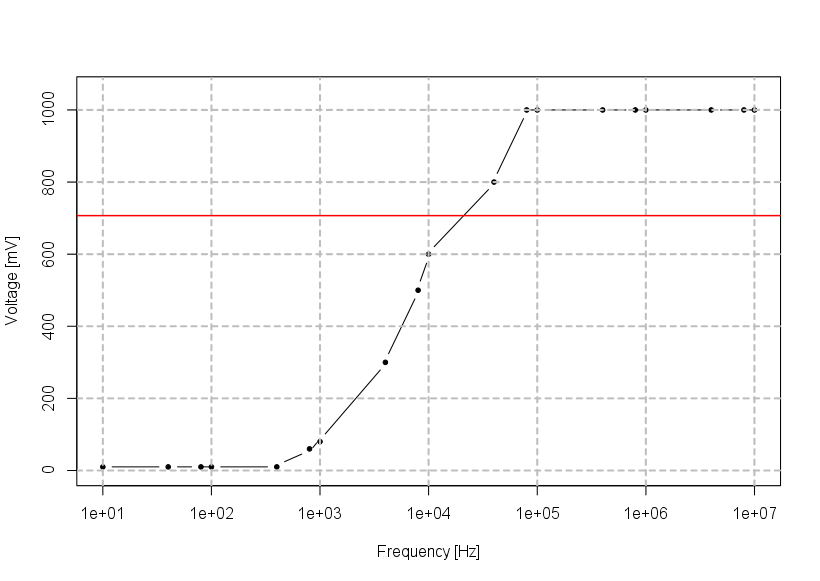
\includegraphics[scale = 0.5]{F:/Projekty Intellij/Text/Metrologia/Ćwiczenie3/Img/Rplot02.png}
    \end{center}
    \par Na podstawie wykresu możemy zaobserwować, że krzywa posiada tylko jeden punkt przecięcia z linią częstotliwości granicznej (czerwona linia).
    Zakładając ze układ, na którym odbywały się pomiary to szeregowy układ RLC wskazywałoby to na posiadanie przez układ tylko składowej C lub L.
    Znając charakterystykę kapacytancji i induktancji możemy od razu zauważyć, że nasz element mierzony blokuje małe częstotliwości co jest w przypadku
    połączenia szeregowego elementów charakterystyczne dla elementów pojemnościowych. Możemy więc wywnioskować, że mierzony układ to dwójnik RC.\\
    \indent Na podstawie wykresu wyznaczamy częstotliwość graniczną na około 33[kHz].
    Moduł impedancji wyliczamy ze wzoru:
    \begin{gather*}
        Z=\sqrt{R^2+(\frac{1}{\omega C})^2}=\sqrt{R^2+(\frac{1}{2\pi f C})^2}
    \end{gather*}
    Częstotliwość graniczna dla filtra górnoprzepustowego wyraża się wzorem:
    \begin{gather*}
        f=\frac{1}{2\pi RC}
    \end{gather*}
%    Zależność współczynnika wzmocnienia dla filtra górnoprzepustowego RC:
%    \begin{gather*}
%        A_v=\frac{V_{out}}{V_{in}}=\frac{R}{Z}=\frac{R}{\sqrt{R^2+X_c^2}}=\frac{R}{Z}=\frac{R}{\sqrt{R^2+(\frac{1}{2\pi fC})^2}}
%    \end{gather*}
    Wzór na impedancję elementu mierzonego stworzony na podstawie wzoru na impedancyjny dzielnik napięcia:
    \begin{gather*}
        Z_L=Z_0(\frac{V_{open}}{V_{loaded}}-1)
    \end{gather*}
    {\footnotesize
        \begin{itemize}
            \setlength\itemsep{0em}
            \item[] \boldmath$Z_L$ - impedancja przy obciążenia,
            \item[] \boldmath$Z_0$ - impedancja nieobciążonego układu(w tym przypadku podana przez producenta),
            \item[] \boldmath$V_{open}$ - napięcie na rozwartym generatorze funkcji,
            \item[] \boldmath$V_{loaded}$ - napięcie na obciążonym generatorze funkcji,
        \end{itemize}}
    \noindent Podstawiając do powyższego wzoru obliczamy impedancję układu mierzonego:
    \begin{gather*}
        Z_L=50[\Omega]\cdot(\frac{1[V]}{0.707946[V]}-1)=20.626\dots[\Omega]
    \end{gather*}
    \par Korzystając ze wzoru na moduł impedancji oraz wzoru na częstotliwość graniczną, które zostały wypisane powyżej, możemy obliczyć składowe R i C
    przy pomocy układu równań. Obliczenie tego układu równań zostało przeprowadzone przy pomocy programu Wolframalpha. Poniżej
    zostały przedstawione wyniki tych kalkulacji:
    \begin{equation*}
        R\approx 14.5848[R]
    \end{equation*}
    \begin{equation*}
        C\approx 0.000000330678[F]=330.678[nF]
    \end{equation*}
    \newpage

    \section{Uwagi i wnioski}
    Ćwiczenie pozwoliło na dokładniejsze zrozumienie doboru metody pomiaru rezystancji od danych warunków eksperymentu.
    Zaczynając od pomiarów przy wykorzystaniu omomierza analogowego możemy zauważyć, że jest on urządzeniem przydatnym w przypadku
    gdy potrzebujemy określić przybliżoną wartość rezystancji elementu mierzonego i gdy nie zależy nam na dużej dokładności.\\
    \indent W przypadku pomiarów od których wymagamy wysokiej precyzji możemy podejść do tego zadania na jeden z trzech sposobów:
    \begin{itemize}
        \setlength\itemsep{0em}
        \item Metodą bezpośrednią - metoda dwu i czteropunktowa,
        \item Metodą pośrednią - poprzez pomiar napięcia i natężenia prądu elektrycznego na elemencie badanym,
        \item Metodą mostkową/zerową - mostek wheatstone`a lub thomsona,
    \end{itemize}
    \par Jeżeli chcemy wykonać pomiar przy wykorzystaniu jak najprostszego układu pomiarowego wskazaną metodą będzie metoda bezpośrednia.
    Większość omomierzy i multimetrów pozwala na tego typu pomiary przy pomocy metody dwupunktowej. Mimo że pomiar ten jest dokładny
    to należy uwzględnić przy nim rezystancję przewodów pomiarowych, które stosujemy. Lepszą alternatywą będzie metoda czteropunktowa.
    Pozwala ona na dokładny pomiar rezystancji bez obawy o wpływ przewodów na układ mierzony. Niestety nie każdy miernik pozwala
    na pomiar przy wykorzystaniu tej metody.\\
    \indent Innym podejściem do pomiaru rezystancji jest metoda pośrednia. Polega ona na jednoczesnym pomiarze napięcia i natężenia na elemencie
    mierzonym. Metoda ta posiada dość skomplikowany układ pomiarowy składający się z dwóch mierników, źródła zasilania oraz elementu mierzonego.
    Dodatkowym problemem tej metody jest określenie topologi układu z uwzględnieniem pozycji mierników. Do określenia jakiej metody
    jaką posłużymy się posłużymy się wartością rezystancji granicznej miernika. Pozwala ona określić nam czy do pomiaru rezystancji należy
    wybrać metodę poprawnego pomiaru napięcia czy metodę poprawnego pomiaru prądu.\\
    \indent Wyżej wymienione metody pozwalają nam na wyróżnienie sposobu dokładnego pomiaru małych i bardzo dużych rezystancji. Jednak warto byłoby
    wspomnieć o jeszcze jednej metodzie niewymienionej w ćwiczeniu. Jest to metoda mostka Thomsona. Jest to metoda mostkowa wykorzystująca
    skomplikowany układ pomiarowy, jednak daje nam przewagę, której nie dają nam żadne inne metody. Pozwala ona na dokładne pomiary rezystancji
    o wartości mniejszej od 1[$\Omega$].
    \newpage
    \subsection*{Uwagi}
    Przy przeprowadzaniu doświadczenia, eksperymentatorzy napotkali kilka problemów, które doprowadziły do pogorszenia wyników ćwiczenia.
    W części 11 gdzie należało skonstruować układ poprawnego pomiaru prądu eksperymentatorzy popełnili błąd przy podłączaniu terminali mierników.
    Spowodowało to to, że rzeczywisty układ jak i został złożony był układem poprawnego pomiaru napięcia. Należy wyciągnąć wnioski, że warto
    wielokrotnie upewniać się co do poprawności zsyntetyzowanego układu pomiarowego oraz że należy sprawdzać, czy wyniki, jakie daje nam metoda
    pomiarowa na pewno pokrywają się z wartościami przewidywanymi.

    %Bibliografia
    \vfill
    \footnotesize
    \begin{thebibliography}{9}
        \bibitem{texbook1}
        https://wzn.pwr.edu.pl/materialy-dydaktyczne/metrologia-elektroniczna
        \bibitem{texbook2}
        https://lpf.wppt.pwr.edu.pl/pomoce-dydaktyczne.php
        \bibitem{texbook3}
        https://www.wolframalpha.com/
        \bibitem{texbook4}
        https://www.keysight.com/us/en/assets/7018-01144/data-sheets/5988-8544.pdf
        \bibitem{texbook5}
        https://en.wikipedia.org/wiki/Electrical-impedance
        \bibitem{texbook6}
        https://en.wikipedia.org/wiki/High-pass-filter
    \end{thebibliography}

\end{document}